\chapter{Fonctionnalités}

\noindent Voici le rendu visuel de l'application, composé de deux contenus principaux, accessible via des onglets :

\begin{figure}[h!]
  \centering
    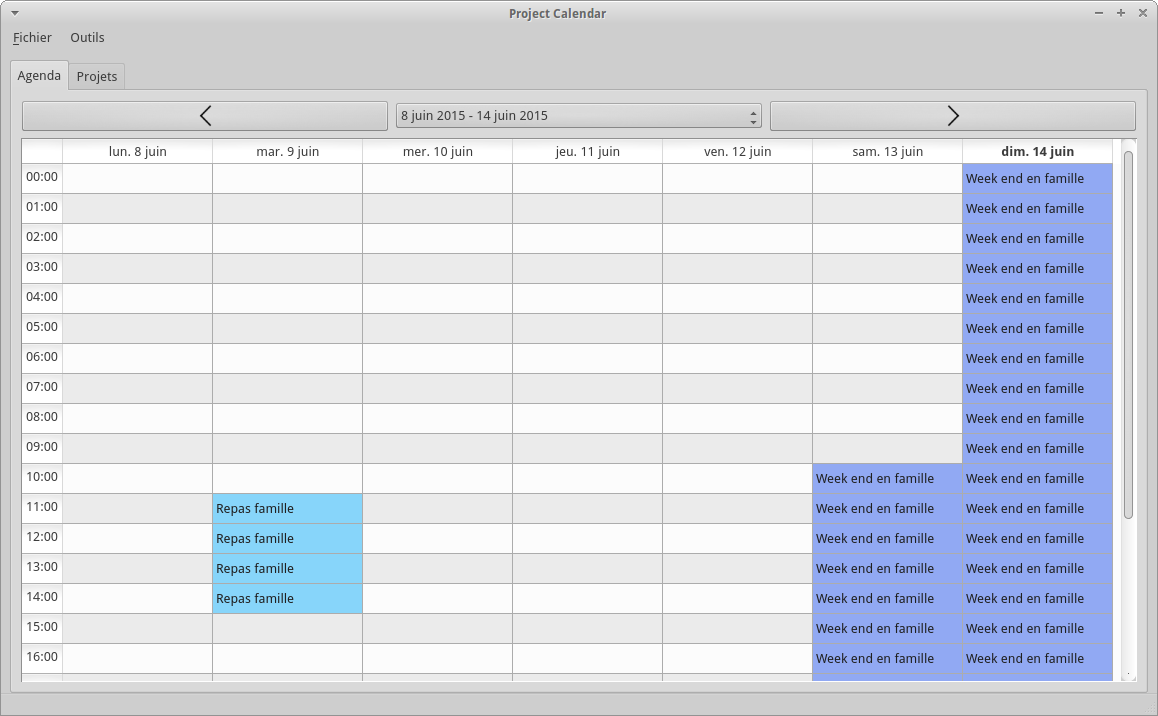
\includegraphics[width=1.0\textwidth]{assets/screen_agenda.png}
    \caption{Partie de l'application dédiée à l'agenda}
\end{figure}

\begin{figure}[h!]
  \centering
    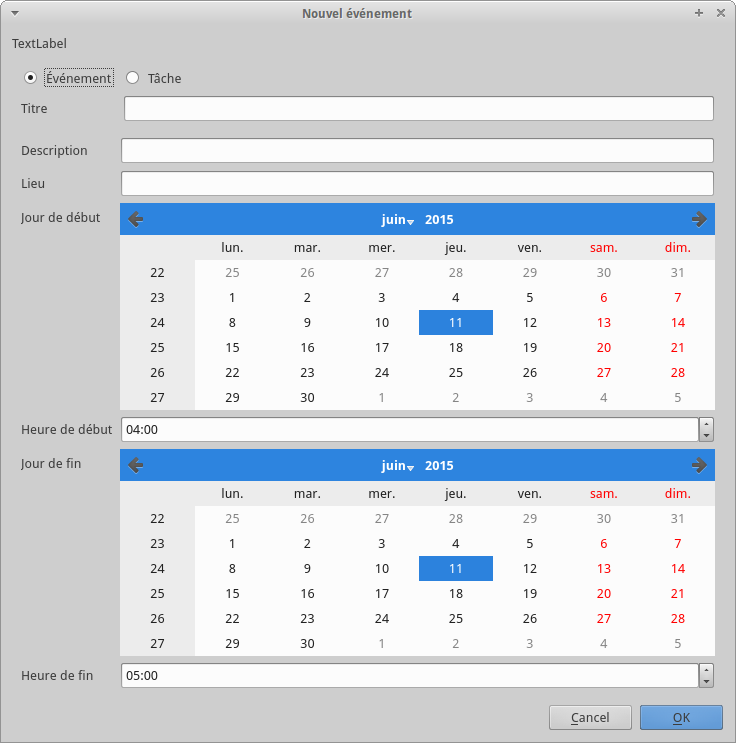
\includegraphics[width=0.49\textwidth]{assets/screen_event.png}
    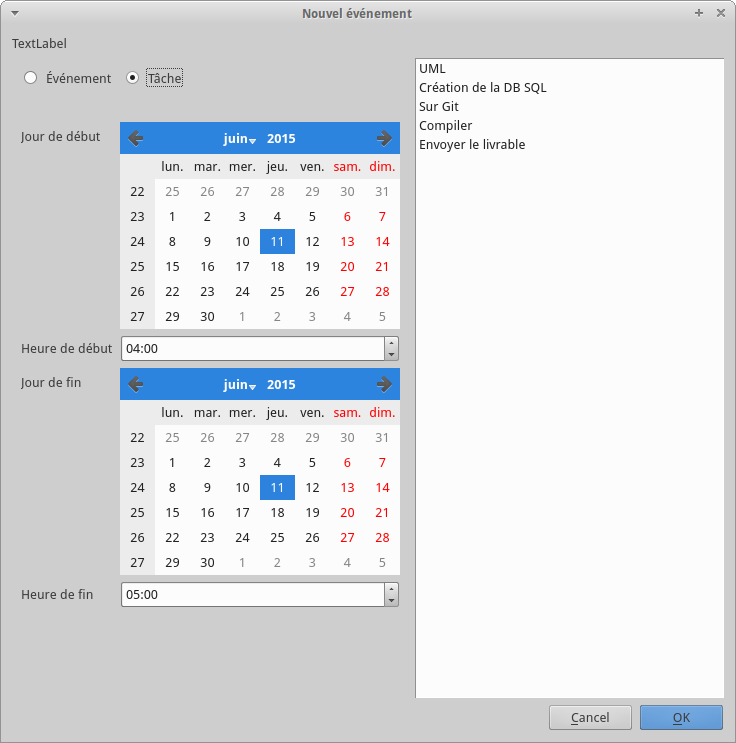
\includegraphics[width=0.49\textwidth]{assets/screen_event_tache.png}
    \caption{Création d'un nouvel événement}
\end{figure}

\begin{figure}[h!]
  \centering
    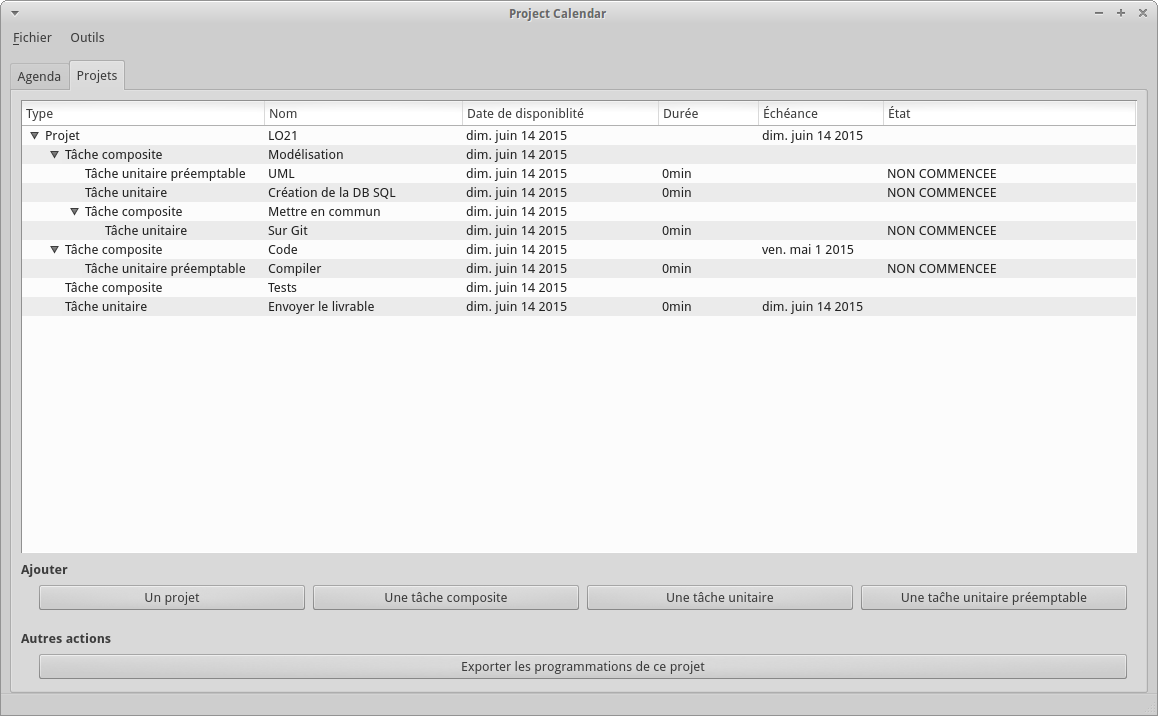
\includegraphics[width=1.0\textwidth]{assets/screen_projets.png}
    \caption{Partie de l'application dédiée aux projets et tâches}
\end{figure}

Nous avons implémenté les fonctionnalités suivantes.

\section{Choix de la semaine à afficher}

Par défaut, la semaine courante est affichée. Le jour courant est en gras. L'utilisateur peut changer la semaine affichée à l'aide d'une liste déroulante (au milieu de l'écran) ou à l'aide des boutons \og Suivant\fg{} et \og Précédent\fg{}.

L'agenda affiche les événements programmée pour la semaine affichée.

\section{Création}
\subsection{D'un événement (une programmation)}

Un clic sur un case de l'agenda permet de programmer un événement (les champs dates et heures sont pré-remplis en fonction de la case cliquée). Des vérifications sont faites (par exemple, un événement doit finir après sa date et heure de début)

\subsection{D'un projet}

Via l'onglet \og Projets\fg{}, l'utilisateur peut créer un nouveau projet.

\subsection{D'une tache composite, unitaire ou unitaire et préemptable}

De la même façon qu'un projet, l'utilisateur peut créer les trois type de tâches. Néanmoins, il doit au préalable avoir sélectionné le projet ou la tâche composite qui va accueillir la nouvelle tâche. Les tâches composites ne peuvent être contenus que dans des projets ou des tâches composites. Les éléments de \og\textit{top-level}\fg{} sont donc les projets.

\section{Modification}

Les attributs des projets et tâches peuvent être modifiés (la durée d'une tâche unitaire par exemple).

\section{Export XML}
\subsection{De la semaine actuellement affichée}

Il est possible, via le menu, d'exporter l'ensemble des programmations de la semaine couramment affichée dans un fichier XML.

\subsection{Des programmations relatives aux tâches d'un projet donné}

On peut également exporter uniquement les événements (tâches programmées) d'un projet selectionné, via un bouton en bas, sur l'interface des projets.

\section{Suppression}

Il est possible via le menu de supprimer soit l'ensemble des événements, soit l'ensemble des tâches et projets. La suppressions d'une tâche entraîne la suppression de sa programmation, s'il y en a une.